\subsection{Komplexe Zahlen}\label{subsec:complex-numbers}

Unter den komplexen Zahlen $\mathbb{C}$ versteht man die nächst größere Zahlenmenge
nach den reellen Zahlen $\mathbb{R}$,
die zusätzlich zu einem Realteil auch einen sogenannten Imaginärteil besitzen.
Sie werden im weiteren Verlauf in der kartesischen Form
$z = a + bi$ dargestellt, wobei $a$ der Realteil und $bi$ der Imaginärteil ist.
Der Buchstabe $i$ steht hierbei für die imaginäre Einheit und
ist definiert durch die Gleichung $i^2 = -1$.

\subsubsection{Multiplikation \& Addition von komplexen Zahlen}
\label{subsubsec:addition-and-multiplication-of-complex-numbers}

Viele Rechenoperationen mit komplexen Zahlen funktionieren anders, als man sie
von den reellen oder natürlichen Zahlen gewohnt ist.
Im Folgenden werden zwei dieser unterschiedlich funktionierenden
Operationen vorgestellt:

Zur Addition zwei komplexer Zahlen addiert man den
Realteil und den Imaginärteil getrennt voneinander und fügt diesen
danach wieder zusammen~\cite[S. 2]{lichtenegger_komplexe_2002}:
$(a_1 + {b_1}i) + (a_2 + {b_2}i) = a_1 + a_2 + (b_1 + b_2)i$.

Um komplexe Zahlen zu multiplizieren, wendet man das Distributivgesetz an,
indem man den zweiten Faktor ebenfalls in seinen Realteil und seinen
Imaginärteil unterteilt und diese jeweils einzeln mit dem ersten Faktor multipliziert
\cite[S. 2f.]{lichtenegger_komplexe_2002}.
Die zwei entstehenden Produkte lassen sich dann wie oben beschrieben addieren.
Bei der Multiplikation mit dem Imaginärteil multipliziert man unter anderem
zwei imaginäre Elemente miteinander.
Da $i^2 = -1$ gilt, entsteht durch diese Multiplikation
ein negatives, aber reales Produkt.
Wie in \hyperref[app:2]{A.2} gezeigt, gilt somit:
$ (a + bi)(c + di) = ac - bd + (bc + ad)i $

Das in der Mandelbrot-Menge häufig angewandte Quadrieren von komplexen Zahlen
lässt sich mit der kartesischen Form ebenfalls herleiten \hyperref[app:3]{[A.3]}.
Für eine gegebene, zu quadrierende, komplexe Zahl $a + bi$ gilt somit:
$(a + bi)^2 = a^2 - b^2 + 2abi$.


Ein illustriertes Beispiel soll beide Rechenoperationen veranschaulichen:

\begin{equation}\label{eq:complex-numbers-example}
  \begin{split}
    (\begingroup\color{red} -3\endgroup + \begingroup\color{blue} 6i\endgroup)^2
      + (\begingroup\color{red} 7\endgroup + \begingroup\color{blue} (-4i)\endgroup) \\
    = (
        (\begingroup\color{red} -3\endgroup \cdot \begingroup\color{red} (-3)\endgroup)
          - (\begingroup\color{red} 6\endgroup \cdot \begingroup\color{red} 6\endgroup)
        + (
          (\begingroup\color{blue} 6\endgroup \cdot \begingroup\color{blue} (-3)\endgroup)
          + (\begingroup\color{blue} -3\endgroup \cdot \begingroup\color{blue} 6\endgroup)
        )i
      )
      + (\begingroup\color{red} 7\endgroup + \begingroup\color{blue} (-4i)\endgroup) \\
    = (\begingroup\color{red} -27\endgroup + \begingroup\color{blue} (-36i)\endgroup)
      + (\begingroup\color{red} 7\endgroup + \begingroup\color{blue} (-4i)\endgroup) \\
    = \begingroup\color{red} -20\endgroup + \begingroup\color{blue} (-40i)\endgroup
  \end{split}
\end{equation}

\subsubsection{Graphische Darstellung komplexer Zahlen}

Komplexe Zahlen können wie Zahlen anderer Zahlenmengen grafisch
dargestellt werden.
Da komplexe Zahlen sowohl aus einem Realteil als auch aus
einem Imaginärteil bestehen, reicht eine Achse nicht aus, um diese darzustellen;
stattdessen braucht man eine Ebene\footnote{
  Ebenfalls unter komplexer Zahlenebene und gaußsche Zahlenebene zu finden.
}.
Diese komplexe Zahlenebene teilt den Realteil auf die waagerechte Achse und
den Imaginärteil auf die horizontale Achse auf.
Eine komplexe Zahl $z = a + bi$ besitzt somit die Koordinaten $ P(a|b)$.

Zusätzlich lässt sich eine komplexe Zahl wie eine reelle Zahl absolut betrachten,
wobei dieser absolute Wert ebenfalls als der Abstand zum Ursprung zu betrachten ist
\cite[S. 3]{lichtenegger_komplexe_2002}.
Aufgrund dessen, dass eine komplexe Zahl aus zwei Komponenten besteht, lässt sich
der Abstand über den Satz des Pythagoras berechnen:

\begin{equation}\label{eq:absolute-complex-number}
  |z|^2 = a^2 + b^2
  \quad
  \text{ beziehungsweise }
  \quad
  |z| = \sqrt{a^2 + b^2}
\end{equation}

\begin{figure}[H]
  \centering
  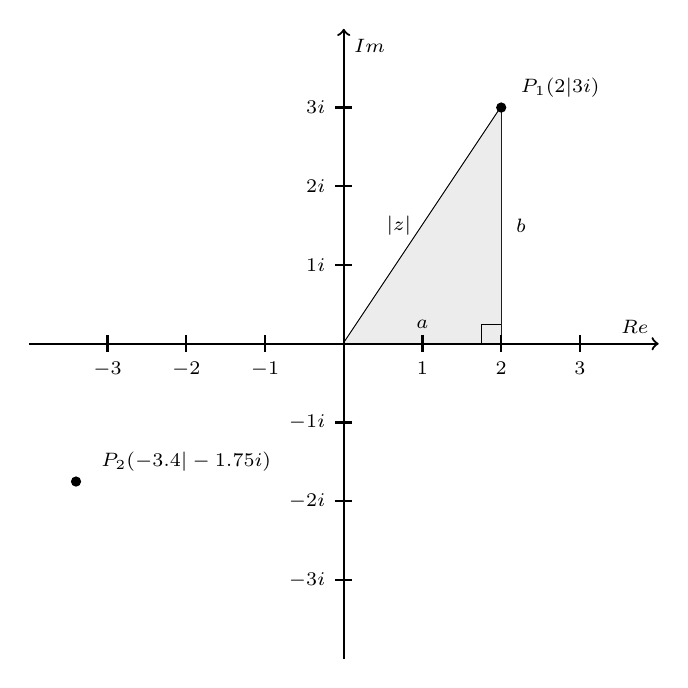
\begin{tikzpicture}
    \begin{scope}[thick,font=\scriptsize]
      \draw (0,0) -- (0,2);
      \draw (2,0) -- (2,3);
      \draw (0,0) -- (2,3);
      \fill[fill=gray!15] (0,0)--(2, 0)--(2,3);
      \node at (1,0.25) {$ a $};
      \node at (2.25,1.5) {$ b $};
      \node at (0.70,1.5) {$ |z| $};
      \draw [line width=0.4pt] (1.75, 0)|-(2, 0.25);

      \draw [fill=black] (2,3) circle(0.05);
      \draw [fill=black] (-3.4, -1.75) circle(0.05);
      \node at (2.75,3.25) {$ P_1(2|3i)$};
      \node at (-2,-1.50) {$ P_2(-3.4|-1.75i)$};

      \draw [->] (-4,0) -- (4,0) node [above left]  {$Re$};
      \draw [->] (0,-4) -- (0,4) node [below right] {$Im$};

      \foreach \n in {-3,...,-1,1,2,...,3}{
        \draw (\n, 3pt) -- (\n, -3pt)   node [below] {$\n$};
        \draw (3pt,\n) -- (-3pt,\n)   node [left] {$\n i$};
      }
    \end{scope}
  \end{tikzpicture}
  \caption{
    Komplexe Ebene mit den Punkten $ P_1, \text{ und } P_2$
    und dem absoluten Wert $|z| \text{ vom Punkt } P_1$.
  }
  \label{fig:complex-numbers-figure-example}
\end{figure}